\documentclass[12pt]{article}
 
\usepackage[margin=1in]{geometry} 
\usepackage{amsmath,amsthm,amssymb}
\usepackage{hyperref}
\usepackage{graphicx}
\usepackage{xcolor}
\usepackage[many]{tcolorbox}
\tcbuselibrary{listings}
\usepackage{listings}
\usepackage{subfig}

\usepackage{float}
\definecolor{lg}{HTML}{f0f0f0}

\newtcblisting{pycode}{
    colback=lg,
    boxrule=0pt,
    arc=0pt,
    outer arc=0pt,
    top=0pt,
    bottom=0pt,
    colframe=white,
    listing only,
    left=15.5pt,
    enhanced,
    listing options={
        basicstyle=\small\ttfamily,
        keywordstyle=\color{blue},
        language=Python,
        showstringspaces=false,
        tabsize=2,
        numbers=left,
        breaklines=true
    },
    overlay={
        \fill[gray!30]
        ([xshift=-3pt]frame.south west)
        rectangle
        ([xshift=11.5pt]frame.north west);
    }
}

\lstset{
    language=Python,
    basicstyle=\small\ttfamily,
}

 
\begin{document}
 
\title{Home Assignment 1}
\author{Cristian Manuel Abrante Dorta - 888248\\
CS-E4650 - Methods of data mining}

\maketitle
\section{Task 1}
\label{sec:task-1}

\subsection{Perform K-means and evaluate the goodness of clustering using
Silhouette Coefficient, Calinski Harabasz and Davies-Bouldin indices.
K = 2.}

An analysis of the results of the K-Means algorithm has been performed for three different values of K, and three indexes respectively. To reproduce the results, the random seed of the generator has been set to the value of $10$, obtaining the following results:

\begin{table}[h]
\centering
\begin{tabular}{c|ccc}
       & Avg. Silhouette coefficient & Calinski-Harabsz index & Davies-Bouldin score \\ \hline
$K = 2$  & 0.5587                 & 847.702                & 0.6216               \\
$K = 5$  & 0.4006                 & 778.4351               & 0.9299               \\
$K = 10$ & 0.3489                 & 593.5482               & 1.0729              \\

\end{tabular}
\caption{Results of different indexes for K = 2, K= 5 and K=10}
\label{tab:coefs}
\end{table}

\subsection{What is the optimal $K$ and why?}
\label{sec:optimal-k}

For answering this question, it is needed analysis of the performance of the K-means algorithm for each index, and each value of $K$.

\subsubsection{Silhouette coefficient}

The silhouette score indicates how each data point is close to the cluster it was matched by the algorithm, and how far it is from the other clusters (the neighbor clusters). This score varies from $[-1, +1]$, and can be calculated for each data point, as it is represented in Figures \ref{fig:sil-k-2}, \ref{fig:sil-k-5}, \ref{fig:sil-k-10}: \\

\begin{figure}[H]
   \begin{minipage}{0.32\textwidth}
     \centering
     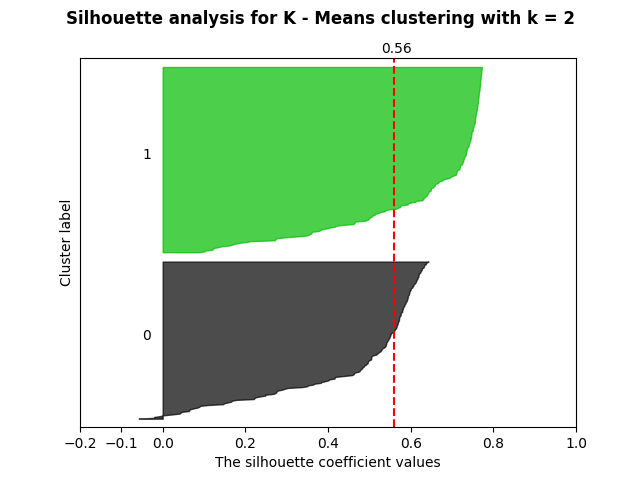
\includegraphics[width=\linewidth]{assignment-1/plots/task-1/silhouette-plot-k-2.png}
     \caption{$K = 2$}
     \label{fig:sil-k-2}
   \end{minipage}\hfill
   \begin{minipage}{0.32\textwidth}
     \centering
     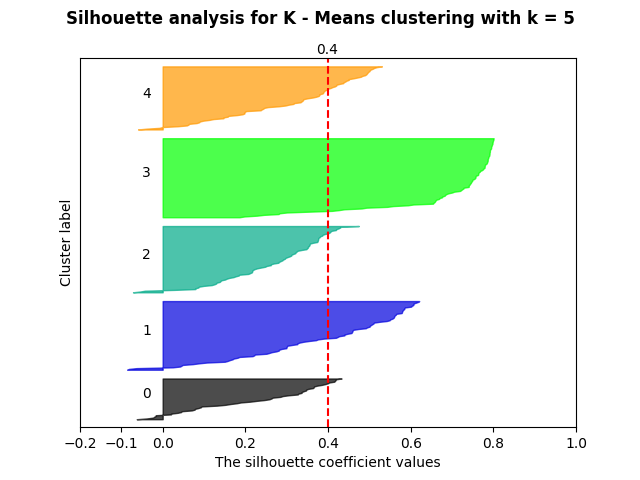
\includegraphics[width=\linewidth]{assignment-1/plots/task-1/silhouette-plot-k-5.png}
     \caption{$K = 5$}
     \label{fig:sil-k-5}
   \end{minipage}
   \begin{minipage}{0.32\textwidth}
     \centering
     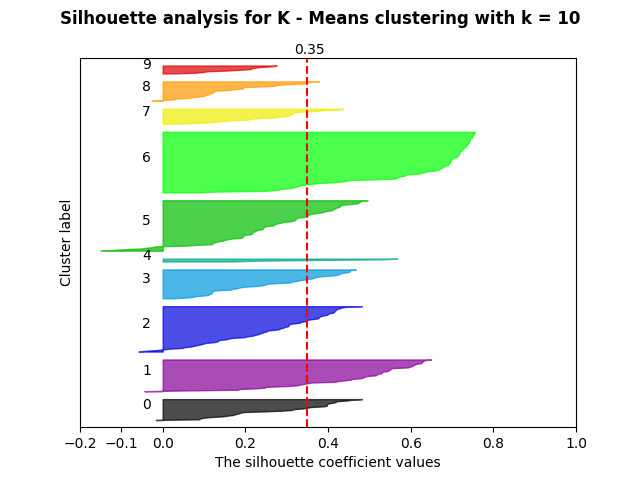
\includegraphics[width=\linewidth]{assignment-1/plots/task-1/silhouette-plot-k-10.png}
     \caption{$K=10$}
     \label{fig:sil-k-10}
   \end{minipage}
\end{figure}

Apart from the silhouette score for each data point, we can calculate the average for all the data points, which is the value shown in the first column of Table \ref{tab:coefs}. \\

The interpretation of the Silhouette score indicates that bigger values are better (close to $+1$), because when a big value is obtained it is an indication that the data points are closer to the cluster that they were assigned by the algorithm. The average score also follows this reasoning, having a better performance when it is higher.\\

If the averages values of the silhouette score are compared (Table \ref{tab:coefs}), it is shown that the value of $K=2$ is the better option with a value of $0.5587$, followed by $K=5$ with a value of $0.4006$ and finally $K=10$ with a value of $0.3489$. This can be also interpreted graphically, in the case of two clusters (Figure \ref{fig:sil-k-2}), we can see that most of the data points are well classified with values bigger than $0$ in almost all cases, except from some data points for cluster 0, which can be considered as outliers. For $K=5$ (Figure \ref{fig:sil-k-5}), there is also a good classification in most of the cases, but there are more points that have values smaller than $0$, on clusters 0,1,2 and 4. Finally, for $K=10$ (Figure \ref{fig:sil-k-10}), which is the worst result obtained in the average score, we can see that there are some points which are not well classified, especially in cluster 5, where some points have negatives values smaller than $-0.1$, also there are some clusters which are not well balanced in the proportion of points, and that is especially important in cluster 4, which do not contain almost data points.

\subsubsection{Calinski-Harabsz index}

This index is not measured for each data point as the silhouette score, but it is a unique value for all the datasets. The results obtained for different values of $K$ can be observed in the second column of Table \ref{tab:coefs}.\\

In the case of the Calinski-Harabsz index, as it indicates the ratio of dispersion between clusters and inter clusters, we can consider that bigger values are better. For our result, we can see that the best result is obtained for $K = 2$ with a value of 847.702, then followed by $K=5$ with a value of 778.4351 and finally $K=10$ with a value of 593.5482.

\subsubsection{Davis-Bouldin Index}

This index is more focused on measuring the separation between the specified clusters, this is why in this case lower values are better because they indicate less separation.\\

The results for this index could be seen in the third column of Table \ref{tab:coefs}. As in the previous indices, the best result is obtained by the execution with $K=2$ with a value of 0.6216, followed by the results of $K=5$ with a value of 0.9299, and finally, the worst performance is obtained by $K=10$ with a value of 1.0729.

\subsubsection{Selection of the optimal $K$}

According to the results obtained by all of the three indices, we can conclude that the best cluster performance is obtained for a value of $K=2$. It has the best performance for all three indices and also in the graphical representation of Figure \ref{fig:fig1}, we can see that almost all the data points are correctly clustered. \\

We can also add that, even though the value of $K=2$ is the one which offers the best performance, maybe for some domains are needed more clusters. In that case, we can say that $K=5$ offers the best trade-off between the number of clusters and evaluation performance.  

\section{Task 2}

\subsection{Perform hierarchical agglomerative clustering using different linkage metrics}

We have performed hierarchical clustering to the dataset using different linkage metrics. For each metric, a dendrogram was generated for showing how data is going to be grouped. Each dendogram is cut in the fourth level, for creating a clearer visualization. 

\begin{figure} [H]
\centering
\subfloat[Single-linkage metric]{
  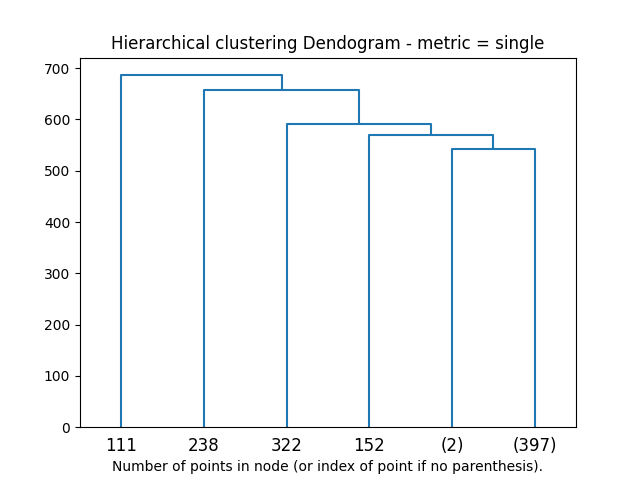
\includegraphics[width=65mm]{assignment-1/plots/task-2/dendogram-single-p4.png}
}
\subfloat[Complete-linkage metric]{
  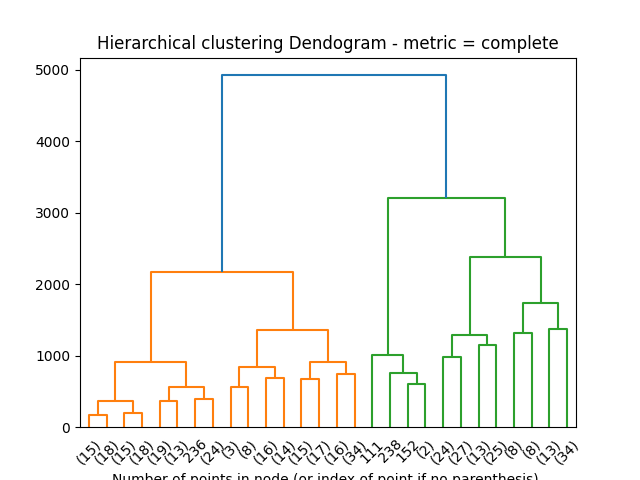
\includegraphics[width=65mm]{assignment-1/plots/task-2/dendogram-complete-p4.png}
}
\hspace{0mm}
\subfloat[Average-linkage metric]{
  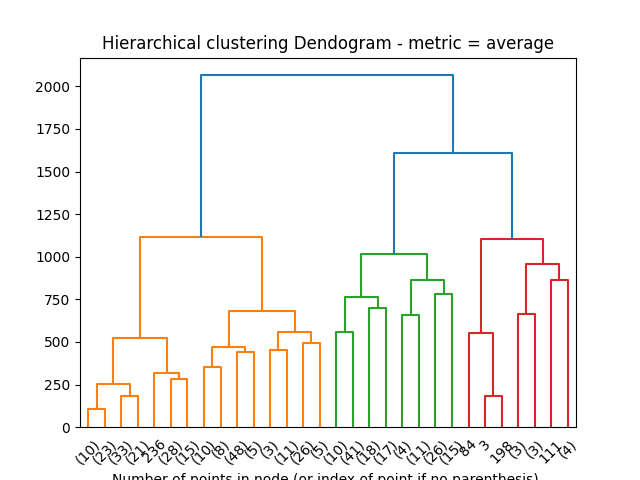
\includegraphics[width=65mm]{assignment-1/plots/task-2/dendogram-average-p4.png}
}
\subfloat[Distance of centroids metric]{
  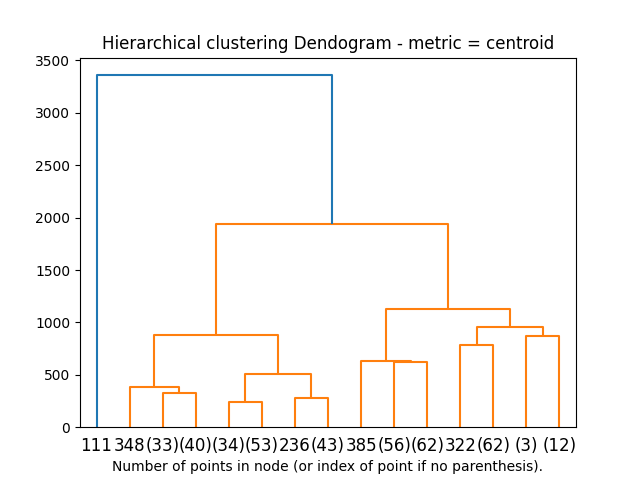
\includegraphics[width=65mm]{assignment-1/plots/task-2/dendogram-centroid-p4.png}
}
\hspace{0mm}
\caption{Dendograms of the resulting clustering for the four metrics}
\label{fig:hierarchical-clusters}
\end{figure}

\subsection{What is the optimal metric for this data and why?}

As in Section \ref{sec:optimal-k}, we have to select which is the algorithm (in this case which is the linkage metric), that performs best for our dataset. We have explored in previous sections three different indices for doing that: silhouette, Calinski-Haranasz, and Davies-Bouldin. To keep things simple, we are going to use in this case the Silhouette index for measuring the goodness of the clustering algorithm with different linkage metrics.

\begin{figure} [H]
\centering
\subfloat[Single-linkage metric]{
  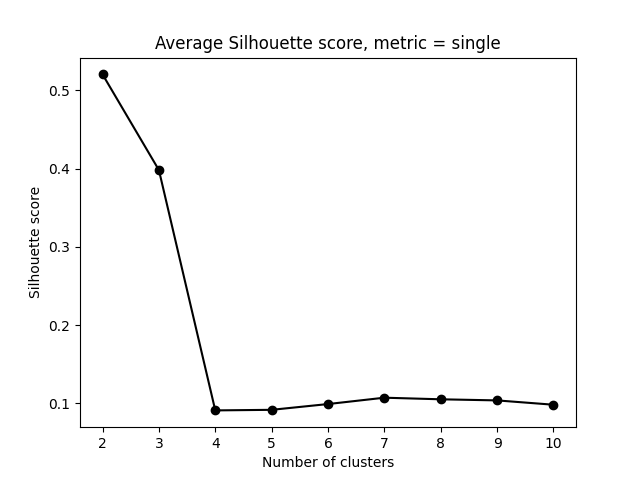
\includegraphics[width=65mm]{assignment-1/plots/task-2/silhouette-single.png}
}
\subfloat[Complete-linkage metric]{
  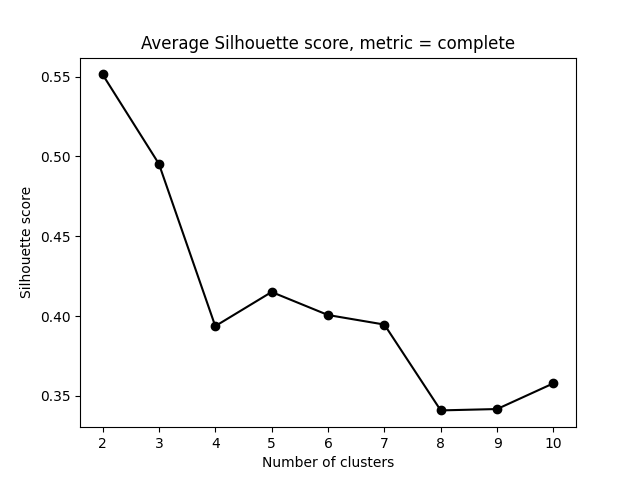
\includegraphics[width=65mm]{assignment-1/plots/task-2/silhouette-complete.png}
}
\hspace{0mm}
\subfloat[Average-linkage metric]{
  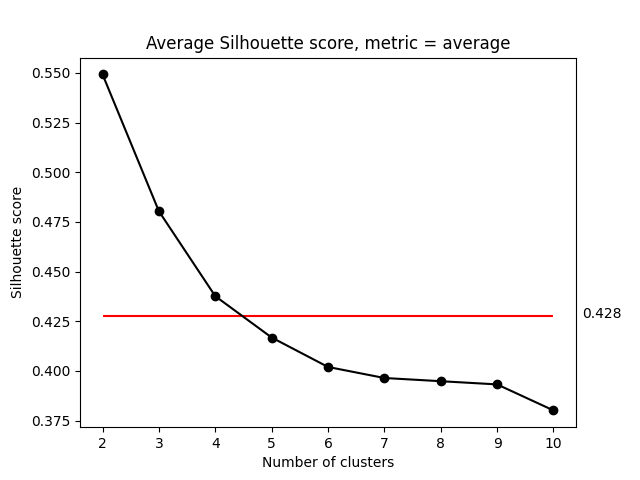
\includegraphics[width=65mm]{assignment-1/plots/task-2/silhouette-average.png}
}
\subfloat[Distance of centroids metric]{
  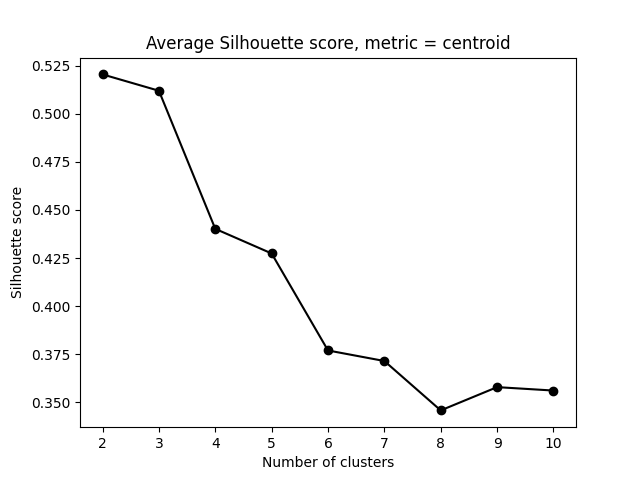
\includegraphics[width=65mm]{assignment-1/plots/task-2/silhouette-centroid.png}
}
\hspace{0mm}
\caption{Plot of the silhouette score for 1 to 10 clusters, for each of the metrics.}
\label{fig:sil-hierarchical}
\end{figure}

In figure \ref{fig:sil-hierarchical} we have created a plot of the performance of the hierarchical cluster algorithm according to silhouette score, with different linkage metrics. Additionally, we have plotted a horizontal line with the average value for all the clusters.\\

According to that, we can say that the metric that has the worst performance is the single metric, with an average score of 0.179, obtaining really bad results when the number of clusters is bigger than 3. With the other metrics, we obtain bigger values (around 0.4), obtaining the best of all them with the average linkage value of 0.428.\\ 

We can not say roundly that this is the best metric, because the other values are really close, but additionally, to have the best result in the metric, we can say that the plot is the most \textit{interpretable} of all of them, because the shape has fewer variations when the number of clusters varies.


\section{Task 2}
To embed code snippets in the report, you can use the \texttt{pycode} environment.

\begin{pycode}
def main():
    print("Hello World")
\end{pycode}

\section{Question 1}

If you add a figure, you can refer to it using Figure.~\ref*{fig:fig1}.

\begin{figure}[h] 
	\centering  % Remember to centre the figure
    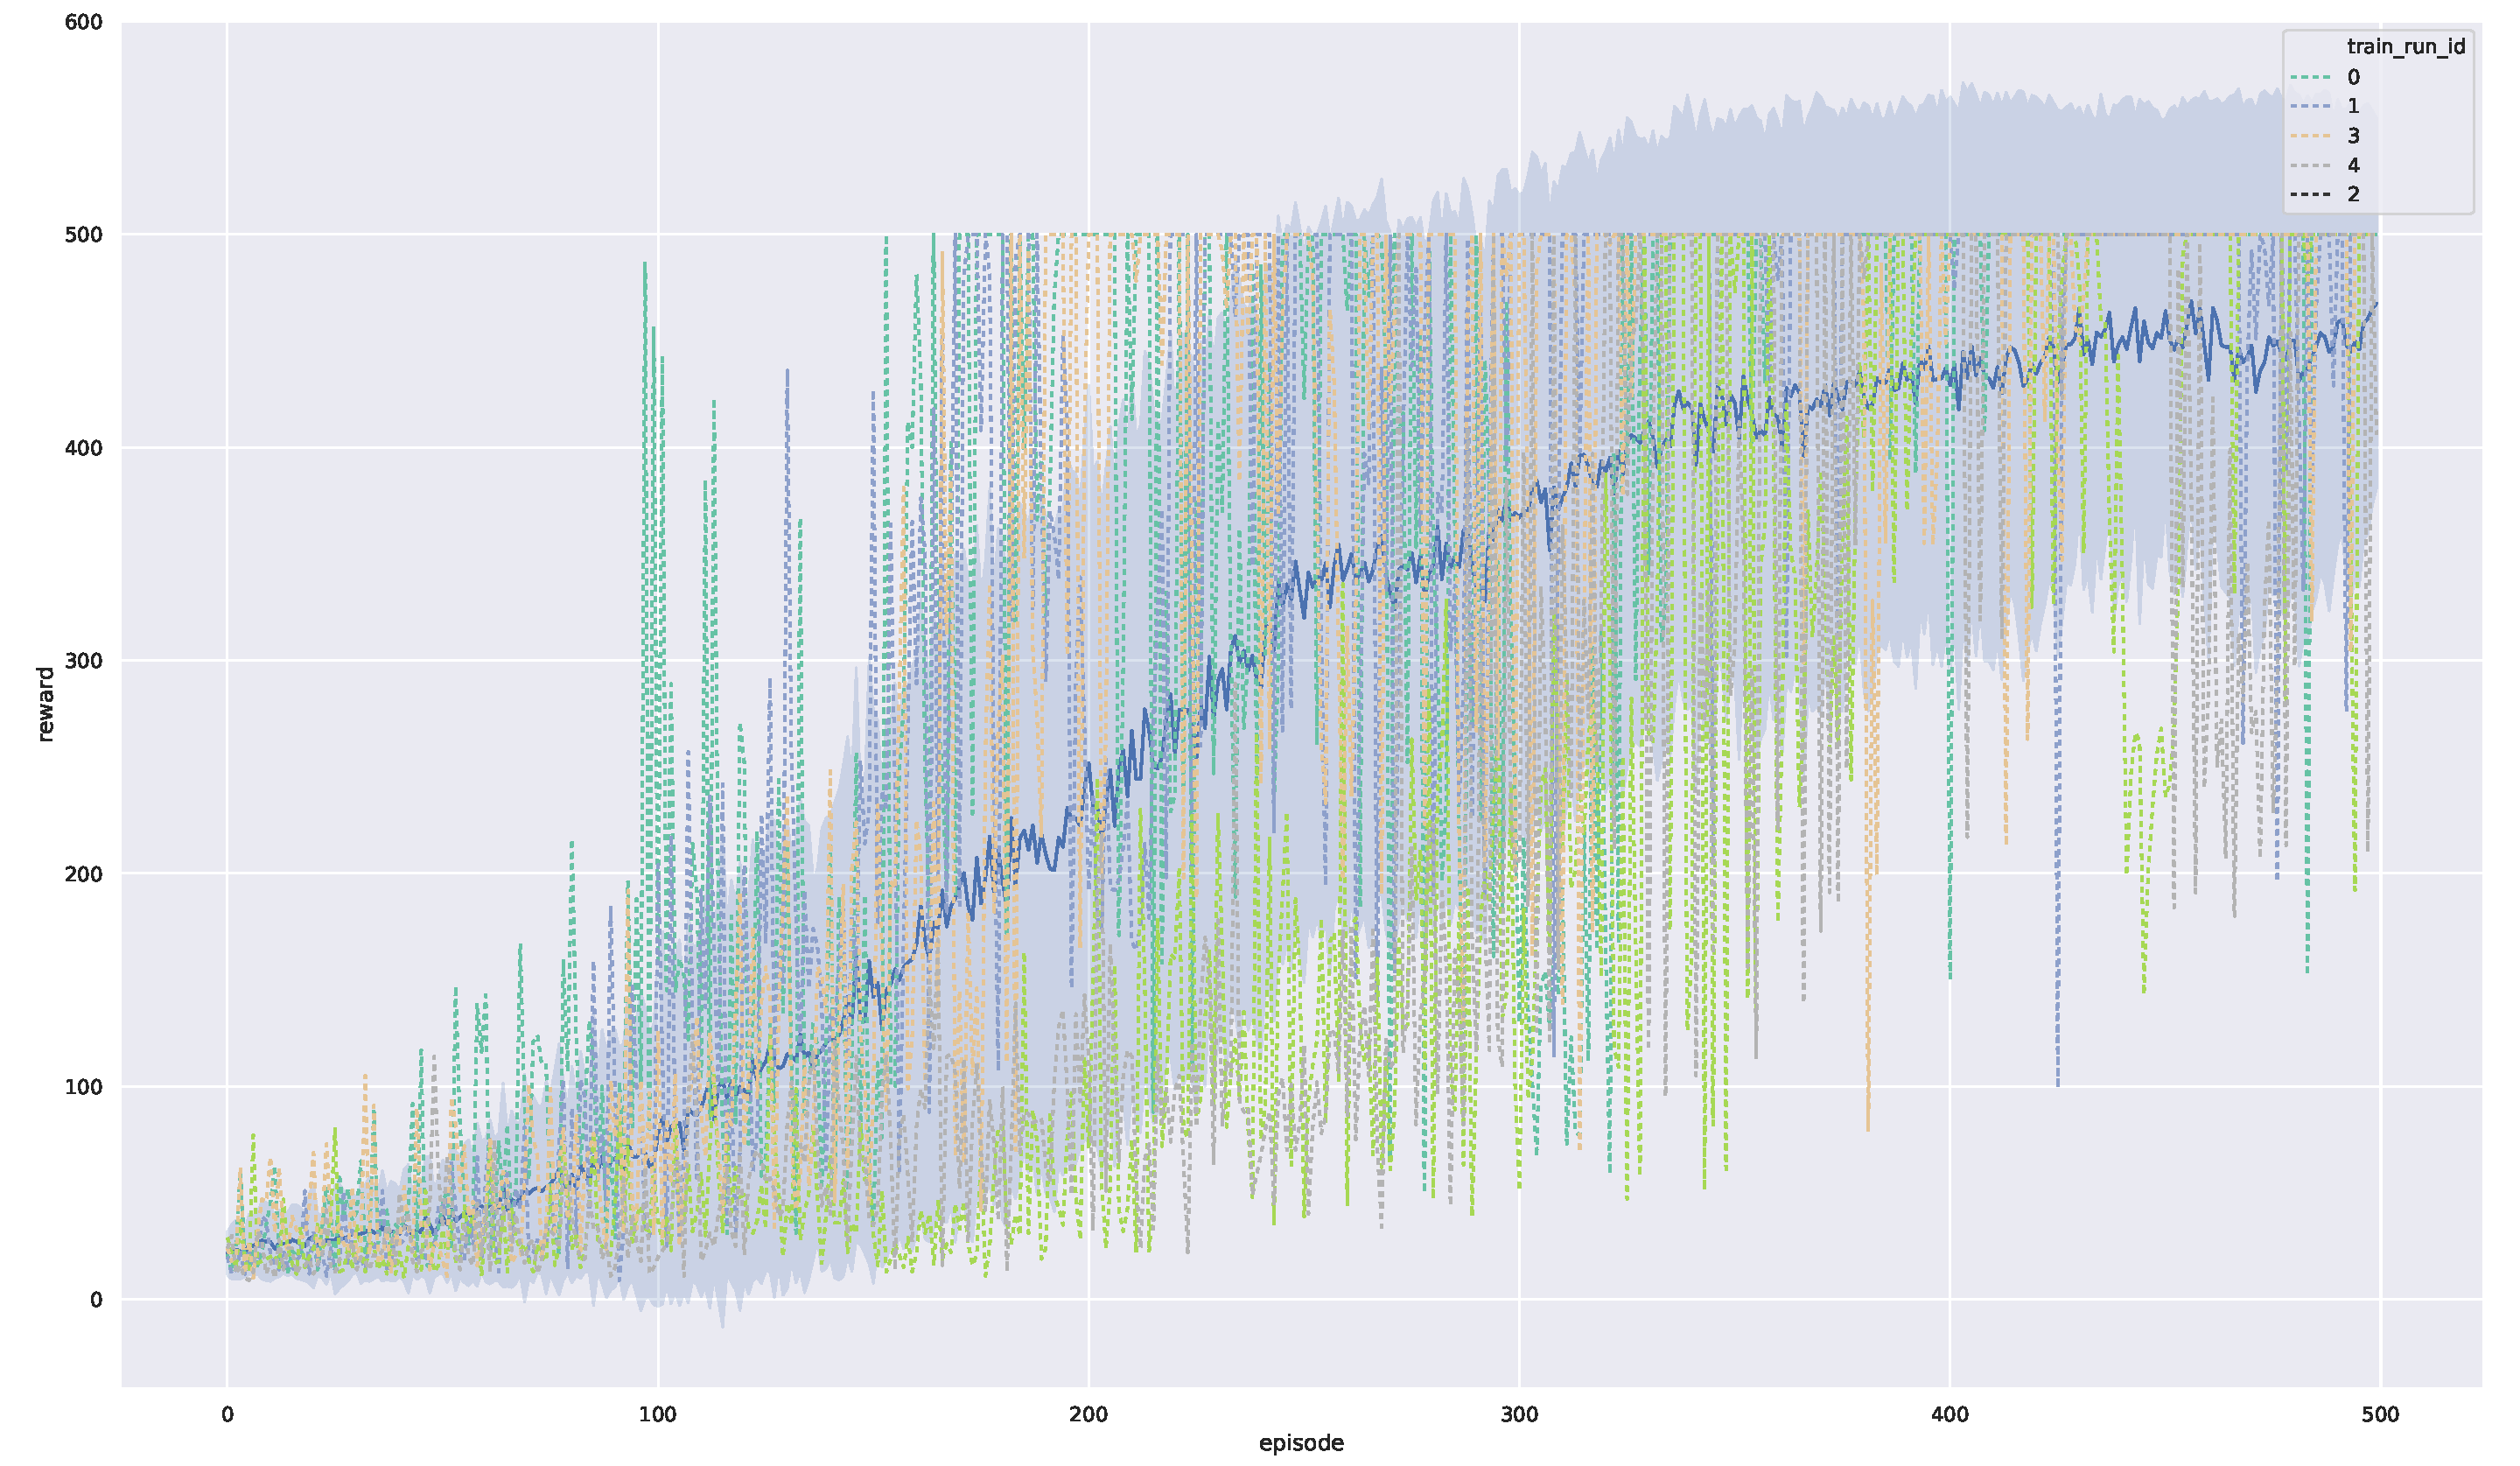
\includegraphics[width=0.3\columnwidth]{img/training.pdf}
	\caption{This is a sample figure.}
	\label{fig:fig1}
\end{figure}

\bibliographystyle{ieeetr}
\bibliography{bibliography}  % Modify template with your bibliography name
\end{document}
